\documentclass[11pt,a4paper]{article}

% ============================================================
%  PACKAGES
% ============================================================
\usepackage[T1]{fontenc}
\usepackage[utf8]{inputenc}
\usepackage[strings]{underscore}      % lets "_" appear naturally in text/headings
\usepackage{mathpazo}                 % elegant Palatino-based body text
\usepackage[scaled=0.90]{helvet}      % Helvetica-like sans for headings
\usepackage[a4paper,margin=2.2cm,top=2.6cm,bottom=2.8cm,headsep=14pt]{geometry}
\usepackage{xcolor}
\usepackage{graphicx}
\usepackage{tikz}
\usepackage{float}
\usetikzlibrary{arrows.meta,positioning,shapes.geometric,fit,backgrounds,decorations.pathreplacing,calc,shadows.blur,shapes.arrows}
\usepackage[most]{tcolorbox}
\tcbuselibrary{skins,breakable,listings,raster}
\usepackage{listings}
\usepackage{fancyhdr}
\usepackage{titlesec}
\usepackage{enumitem}
\usepackage{microtype}
\usepackage{booktabs}
\usepackage{longtable}
\usepackage{tabularx}
\usepackage{colortbl}
\usepackage{multirow}
\usepackage{makecell}
\usepackage{tocloft}
\usepackage{hyperref}
\usepackage{xurl}
\usepackage{needspace}
\usepackage{caption}
\usepackage{changepage}

% ============================================================
%  COLOUR PALETTE
% ============================================================
\definecolor{navy}{RGB}{15,23,42}
\definecolor{navylight}{RGB}{30,41,59}
\definecolor{teal}{RGB}{13,148,136}
\definecolor{tealdark}{RGB}{8,102,94}
\definecolor{amber}{RGB}{217,119,6}
\definecolor{amberlight}{RGB}{254,243,220}
\definecolor{codebg}{RGB}{248,250,252}
\definecolor{codeborder}{RGB}{203,213,225}
\definecolor{titlebar}{RGB}{30,41,59}
\definecolor{softgray}{RGB}{100,116,139}
\definecolor{palegray}{RGB}{241,245,249}
\definecolor{success}{RGB}{21,128,61}
\definecolor{successbg}{RGB}{220,252,231}
\definecolor{danger}{RGB}{185,28,28}
\definecolor{dangerbg}{RGB}{254,226,226}
\definecolor{infobg}{RGB}{224,242,254}
\definecolor{infoborder}{RGB}{14,165,233}
\definecolor{pykw}{RGB}{147,51,234}
\definecolor{pystr}{RGB}{22,163,74}
\definecolor{pycom}{RGB}{100,116,139}
\definecolor{pyfun}{RGB}{8,102,94}

\newcommand{\dotmark}[1]{\raisebox{0.05em}{\tikz[baseline]{\fill[#1] (0,0) circle (2.4pt);}}}

% ============================================================
%  HYPERREF
% ============================================================
\hypersetup{
    colorlinks=true,
    linkcolor=tealdark,
    citecolor=tealdark,
    urlcolor=teal,
    pdftitle={The Agentic RAG Engine --- Architecture \& Implementation Reference},
    pdfauthor={Agentic RAG Engine Project},
    pdfsubject={LangGraph + Model Context Protocol Tool-Agent Architecture},
    bookmarksopen=true,
    bookmarksnumbered=true
}

% ============================================================
%  SECTION TITLE STYLING
% ============================================================
\titleformat{\section}
  {\normalfont\sffamily\Large\bfseries\color{navy}}
  {\colorbox{teal}{\makebox[0.9em]{\color{white}\thesection}}}{0.6em}{}
  [\vspace{2pt}{\color{teal}\titlerule[1.4pt]}]
\titlespacing*{\section}{0pt}{22pt}{14pt}

\titleformat{\subsection}
  {\normalfont\sffamily\large\bfseries\color{tealdark}}
  {\thesubsection}{0.6em}{}
  [{\color{codeborder}\titlerule[0.6pt]}]
\titlespacing*{\subsection}{0pt}{16pt}{8pt}

\titleformat{\subsubsection}
  {\normalfont\sffamily\normalsize\bfseries\color{navylight}}
  {\thesubsubsection}{0.5em}{}
\titlespacing*{\subsubsection}{0pt}{12pt}{6pt}

% ============================================================
%  HEADER / FOOTER
% ============================================================
\pagestyle{fancy}
\fancyhf{}
\renewcommand{\headrulewidth}{0.8pt}
\renewcommand{\footrulewidth}{0.4pt}
\fancyhead[L]{\small\sffamily\color{softgray}Agentic RAG Engine}
\fancyhead[R]{\small\sffamily\color{softgray}\nouppercase{\leftmark}}
\fancyfoot[L]{\small\sffamily\color{softgray}MCP Tool-Agent Architecture}
\fancyfoot[C]{}
\fancyfoot[R]{\small\sffamily\color{softgray}Page \thepage\ of \pageref{LastPage}}
\renewcommand{\headrule}{\hbox to\headwidth{\color{teal}\leaders\hrule height \headrulewidth\hfill}}

% ============================================================
%  TABLE OF CONTENTS STYLING
% ============================================================
\renewcommand{\cftsecfont}{\sffamily\bfseries\color{navy}}
\renewcommand{\cftsecpagefont}{\sffamily\color{teal}}
\renewcommand{\cftsubsecfont}{\sffamily\color{navylight}}
\renewcommand{\cftsubsecpagefont}{\sffamily\color{softgray}}
\setlength{\cftbeforesecskip}{7pt}
\renewcommand{\cftsecleader}{\cftdotfill{\cftdotsep}}
\renewcommand{\contentsname}{\textcolor{navy}{Table of Contents}}

% ============================================================
%  CODE LISTING STYLE (Python / Bash) via listings, wrapped by tcolorbox
% ============================================================
\lstdefinestyle{pystyle}{
    language=Python,
    backgroundcolor=\color{codebg},
    basicstyle=\ttfamily\small,
    keywordstyle=\color{pykw}\bfseries,
    stringstyle=\color{pystr},
    commentstyle=\color{pycom}\itshape,
    numberstyle=\tiny\color{softgray},
    numbers=left,
    numbersep=8pt,
    breaklines=true,
    breakatwhitespace=false,
    showstringspaces=false,
    tabsize=4,
    frame=none,
    xleftmargin=0pt,
    columns=fullflexible,
    keepspaces=true,
    literate={->}{{$\rightarrow$}}1 {\_}{{\_}}1
}
\lstdefinestyle{bashstyle}{
    language=bash,
    backgroundcolor=\color{navy},
    basicstyle=\ttfamily\small\color{white},
    keywordstyle=\color{amber}\bfseries,
    stringstyle=\color{teal},
    commentstyle=\color{softgray}\itshape,
    breaklines=true,
    showstringspaces=false,
    numbers=none,
    columns=fullflexible,
}

\newtcblisting{pycode}[1][]{
    enhanced, breakable, listing only,
    listing options={style=pystyle},
    colframe=codeborder, colback=codebg,
    boxrule=0.6pt, arc=2mm, top=1mm, bottom=1mm,
    fonttitle=\sffamily\bfseries\small,
    coltitle=white, colbacktitle=titlebar,
    attach boxed title to top left={yshift=-2mm,xshift=4mm},
    boxed title style={colback=titlebar, arc=1.5mm, boxrule=0pt},
    title={\dotmark{white}\ #1}
}

\newtcbox{\inlinefile}{on line, arc=1pt, colback=palegray, colframe=codeborder,
    boxrule=0.4pt, boxsep=0pt, left=3pt, right=3pt, top=1pt, bottom=1pt,
    fontupper=\ttfamily\small\color{tealdark}}

% ============================================================
%  CALLOUT BOXES
% ============================================================
\newtcolorbox{infobox}[1][Note]{
    enhanced, breakable, colback=infobg, colframe=infoborder,
    boxrule=0.8pt, arc=2mm, left=8pt, right=8pt, top=6pt, bottom=6pt,
    fonttitle=\sffamily\bfseries, coltitle=infoborder,
    title={\dotmark{infoborder}\ #1}
}
\newtcolorbox{successbox}[1][Verified]{
    enhanced, breakable, colback=successbg, colframe=success,
    boxrule=0.8pt, arc=2mm, left=8pt, right=8pt, top=6pt, bottom=6pt,
    fonttitle=\sffamily\bfseries, coltitle=success,
    title={\dotmark{success}\ #1}
}
\newtcolorbox{warnbox}[1][Design Decision]{
    enhanced, breakable, colback=amberlight, colframe=amber,
    boxrule=0.8pt, arc=2mm, left=8pt, right=8pt, top=6pt, bottom=6pt,
    fonttitle=\sffamily\bfseries, coltitle=amber!70!black,
    title={\dotmark{amber}\ #1}
}
\newtcolorbox{dangerbox}[1][Security]{
    enhanced, breakable, colback=dangerbg, colframe=danger,
    boxrule=0.8pt, arc=2mm, left=8pt, right=8pt, top=6pt, bottom=6pt,
    fonttitle=\sffamily\bfseries, coltitle=danger,
    title={\dotmark{danger}\ #1}
}
\newtcolorbox{filecard}[2]{
    enhanced, breakable, colback=white, colframe=navylight,
    boxrule=0.9pt, arc=1.5mm, left=8pt, right=8pt, top=6pt, bottom=6pt,
    fonttitle=\sffamily\bfseries\small, coltitle=white, colbacktitle=navylight,
    title={\dotmark{white}\ \texttt{#1} \hfill \small\normalfont #2}
}

% ============================================================
%  MISC
% ============================================================
\setlist[itemize]{leftmargin=1.4em, itemsep=2pt, topsep=3pt}
\setlist[enumerate]{leftmargin=1.6em, itemsep=2pt, topsep=3pt}
\renewcommand{\arraystretch}{1.25}
\captionsetup{font=small,labelfont={sf,bf,color=teal},skip=6pt}

\newcommand{\pkgtitle}{The Agentic RAG Engine}
\newcommand{\pkgsub}{Architecture, Retrieval Pipeline \& the Model Context Protocol Tool-Agent Layer}

\usepackage{lastpage}

\begin{document}

% ============================================================
%  TITLE PAGE
% ============================================================
\begin{titlepage}
\newgeometry{margin=0cm}
\begin{tikzpicture}[remember picture, overlay]
    \fill[navy] (current page.north west) rectangle ([yshift=-9.2cm]current page.north east);
    \fill[teal] ([yshift=-9.2cm]current page.north west) rectangle ([yshift=-9.35cm]current page.north east);
    \foreach \x/\y/\r in {2/3/0.55, 4.2/6.5/0.35, 17/2/0.4, 18.5/6/0.6, 15.5/8/0.28}
      \fill[white, opacity=0.05] ($(current page.north west)+(\x,-\y)$) circle (\r);

    \node[anchor=north west, text width=15.5cm, align=left] at ([xshift=2.0cm,yshift=-2.6cm]current page.north west)
      {\color{teal!60!white}\sffamily\bfseries\Large MCP-POWERED TOOL-AGENT ARCHITECTURE};

    \node[anchor=north west, text width=16.5cm, align=left] at ([xshift=2.0cm,yshift=-3.6cm]current page.north west)
      {\color{white}\sffamily\bfseries\fontsize{34}{40}\selectfont \pkgtitle};

    \node[anchor=north west, text width=15.5cm, align=left] at ([xshift=2.0cm,yshift=-5.9cm]current page.north west)
      {\color{white!85!black}\sffamily\large \pkgsub};

    \node[anchor=north west] at ([xshift=2.0cm,yshift=-8.2cm]current page.north west)
      {\color{teal!70!white}\rule{15.5cm}{1.2pt}};

    \node[anchor=north west, text width=16cm, align=left] at ([xshift=2.0cm,yshift=-8.6cm]current page.north west)
      {\color{white!70!black}\sffamily\small LangGraph\ $\cdot$\ Model Context Protocol (official \texttt{mcp} SDK)\ $\cdot$\ BM25 + FAISS + RRF + Cross-Encoder Retrieval};

    % small architecture glyph: three connected nodes
    \begin{scope}[shift={(15.6,-1.9)}]
      \node[circle,draw=white,fill=navylight,minimum size=0.65cm,thick] (g1) at (0,0) {};
      \node[circle,draw=white,fill=teal,minimum size=0.65cm,thick] (g2) at (1.15,0.35) {};
      \node[circle,draw=white,fill=amber,minimum size=0.65cm,thick] (g3) at (1.15,-0.55) {};
      \draw[white,thick] (g1) -- (g2);
      \draw[white,thick] (g1) -- (g3);
      \draw[white,thick] (g2) -- (g3);
    \end{scope}
\end{tikzpicture}

\vspace*{10.6cm}
\begin{center}
{\sffamily\Large\color{navy}\textbf{Technical Reference \& Codebase Deep-Dive}}\\[6pt]
{\sffamily\color{softgray}Covering the retrieval core, the LangGraph multi-agent graph,\\
the standalone MCP server \& client, dynamic tool routing, and resilience design}
\end{center}

\vfill
\begin{center}
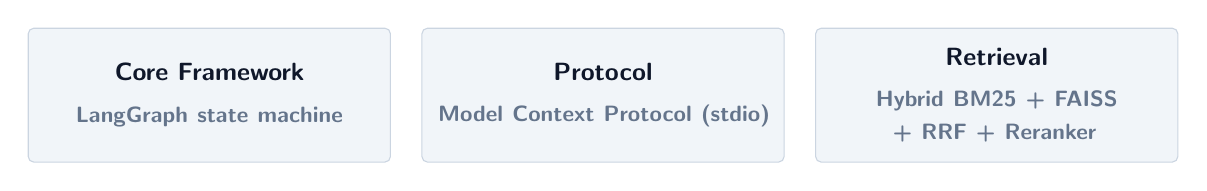
\begin{tikzpicture}
  \foreach \i/\lbl/\sub in {0/Core Framework/LangGraph state machine, 1/Protocol/Model Context Protocol (stdio), 2/Retrieval/Hybrid BM25 + FAISS + RRF + Reranker} {
    \node[draw=codeborder, fill=palegray, rounded corners=2pt, minimum width=4.6cm, minimum height=1.7cm, align=center, text width=4.2cm]
      at (\i*5.0cm,0) {\sffamily\small\bfseries\color{navy}\lbl\\[3pt]\sffamily\footnotesize\color{softgray}\sub};
  }
\end{tikzpicture}
\end{center}

\vspace{1.2cm}
\begin{center}
{\sffamily\small\color{softgray} Prepared for \textbf{\color{navy}Hamdan} \quad$\bullet$\quad Agentic RAG Engine Project \quad$\bullet$\quad \today}
\end{center}
\restoregeometry
\end{titlepage}

\clearpage
\pagenumbering{roman}
\tableofcontents
\clearpage
\pagenumbering{arabic}



\section{Introduction}
\label{sec:intro}

The \textbf{Agentic RAG Engine} is a retrieval-augmented generation system that
diagnoses \emph{why a repository's CI/CD pipeline, Dockerfile, or test suite is
broken} by combining a hybrid retrieval core with a self-correcting,
multi-agent reasoning loop built on \textbf{LangGraph}. Rather than a single
prompt-and-answer call, the engine plans a search, retrieves evidence,
critiques its own evidence for sufficiency, and only then synthesizes a
grounded, cited answer -- retrying with a refined query (or a different
retrieval tool) whenever the evidence falls short.

This document is a complete technical reference for the project as it stands
today: the original hybrid retrieval pipeline, the LangGraph agent graph that
orchestrates it, and its most recent evolution -- exposing that retrieval
pipeline through a real \textbf{Model Context Protocol (MCP)} server, and
replacing a single hardcoded retrieval call with an LLM-driven
\textbf{Tool Agent} capable of dynamically choosing between three different
retrieval tools.

\begin{infobox}[What problem does this solve?]
Given a natural-language question like \textit{"Why does the Docker build
fail?"}, the engine must locate the exact broken configuration inside a
repository, distinguish the \emph{root cause} from the \emph{symptom}, and
produce a minimal, evidence-grounded fix -- without hallucinating file names,
paths, or commands that were never actually retrieved.
\end{infobox}

\subsection{Design Philosophy}

Four principles run through every layer of this codebase:

\begin{enumerate}
\item \textbf{Retrieval algorithms are never duplicated.} BM25, FAISS,
      Reciprocal Rank Fusion, and cross-encoder reranking each live in
      exactly one place; every consumer (the standalone script, the MCP
      server) calls the same shared functions.
\item \textbf{Every external call degrades gracefully.} A missing file, an
      empty search result, a crashed subprocess, or a malformed response
      is always converted into a structured
      \texttt{\{"success": false, "error": "..."\}} shape -- the graph
      never crashes because retrieval came back empty.
\item \textbf{The agent graph stays legible.} \texttt{START} $\rightarrow$
      \texttt{Planner} $\rightarrow$ \texttt{Tool Agent} $\rightarrow$
      \texttt{Critic} $\rightarrow$ \texttt{Router} $\rightarrow$
      \texttt{Synthesizer} $\rightarrow$ \texttt{END} is a fixed, auditable
      shape; new capability is added \emph{inside} a node, not by
      redesigning the graph.
\item \textbf{Tool selection is dynamic, not hardcoded.} The set of
      retrieval tools is discovered at runtime from the MCP server and
      bound to the LLM as real function-calling schemas -- the graph code
      itself contains no \texttt{if tool == "search\_documents"} branching.
\end{enumerate}

\clearpage
\section{High-Level Architecture}
\label{sec:architecture}

Figure~\ref{fig:bigpicture} shows the complete request lifecycle: a user
question enters the LangGraph state machine, the \texttt{Planner} turns it
into a targeted search query, the \texttt{Tool Agent} chooses and executes an
MCP tool, the \texttt{Critic} judges the evidence, and the \texttt{Router}
either loops back for another attempt or hands off to the
\texttt{Synthesizer} for a final, cited answer.

\begin{figure}[h!]
\centering
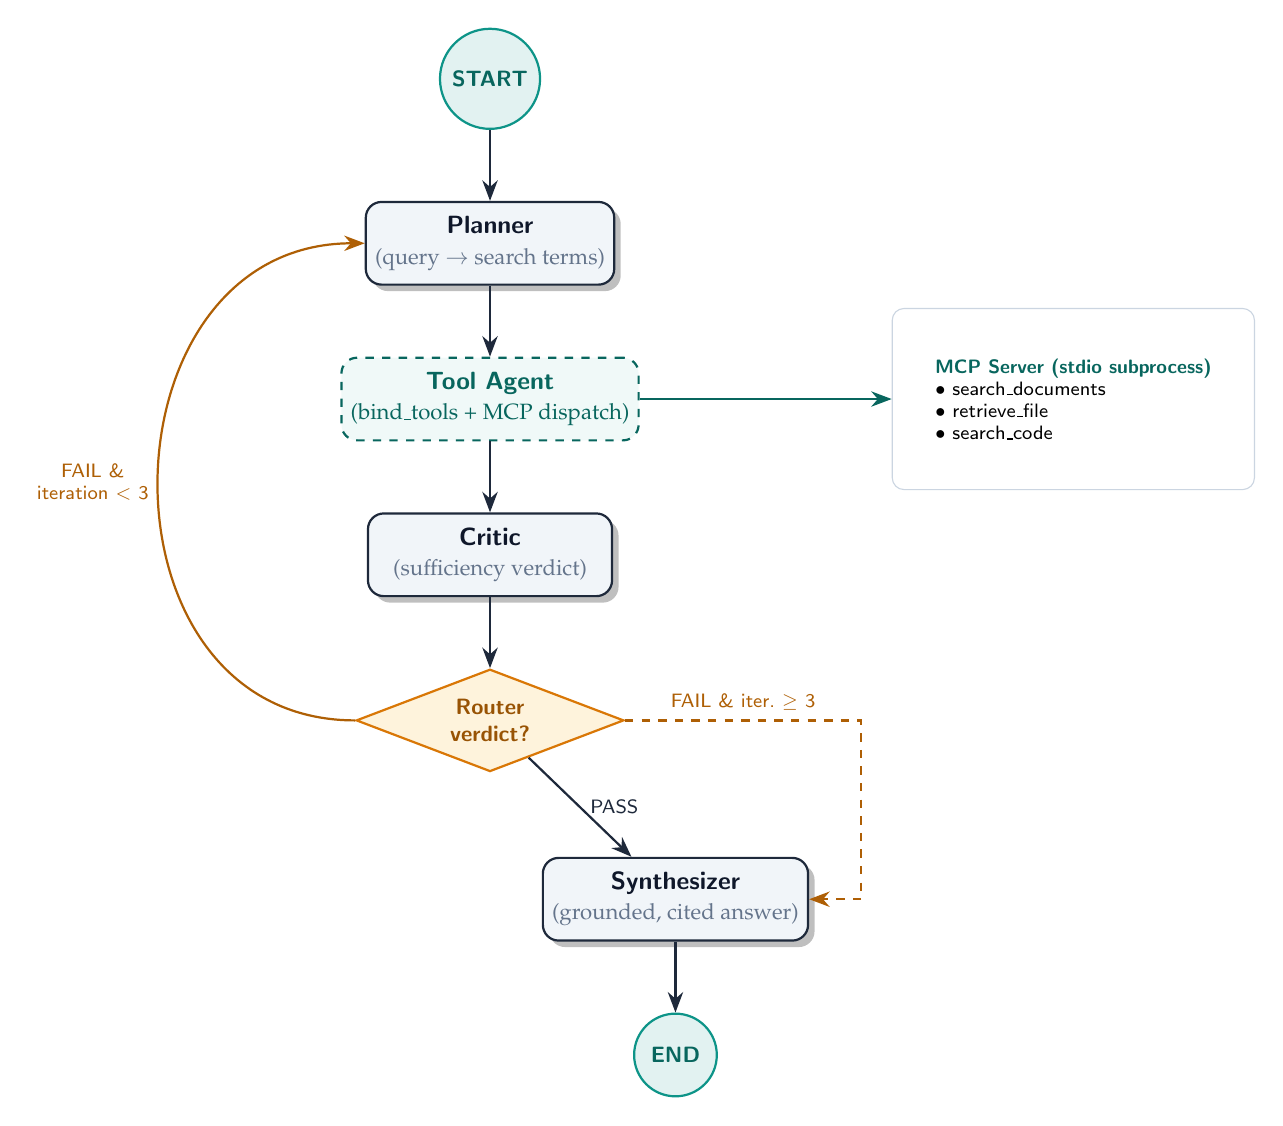
\begin{tikzpicture}[
    node distance=9mm and 18mm,
    box/.style={draw=navylight, thick, rounded corners=2mm, fill=palegray,
                minimum width=3.1cm, minimum height=1.05cm, align=center,
                font=\sffamily\small\bfseries\color{navy}, drop shadow},
    startend/.style={draw=teal, thick, circle, fill=teal!12, minimum size=1.05cm,
                font=\sffamily\footnotesize\bfseries\color{tealdark}},
    decision/.style={draw=amber, thick, diamond, aspect=2.2, fill=amberlight,
                minimum width=3.4cm, minimum height=1.3cm, align=center,
                font=\sffamily\footnotesize\bfseries\color{amber!70!black}, inner sep=1pt},
    mcpbox/.style={draw=tealdark, thick, dashed, rounded corners=2mm, fill=teal!6,
                minimum width=3.6cm, minimum height=1.05cm, align=center,
                font=\sffamily\small\bfseries\color{tealdark}},
    arr/.style={-{Stealth[length=2.6mm]}, thick, navylight},
    loopArr/.style={-{Stealth[length=2.6mm]}, thick, amber!80!black}
]
\node[startend] (start) {START};
\node[box, below=of start] (planner) {Planner\\ \footnotesize\normalfont\color{softgray}(query $\to$ search terms)};
\node[mcpbox, below=of planner] (toolagent) {Tool Agent\\ \footnotesize\normalfont\color{tealdark}(bind\_tools + MCP dispatch)};
\node[box, below=of toolagent] (critic) {Critic\\ \footnotesize\normalfont\color{softgray}(sufficiency verdict)};
\node[decision, below=of critic] (router) {Router\\ verdict?};
\node[box, below right=14mm and -2mm of router] (synth) {Synthesizer\\ \footnotesize\normalfont\color{softgray}(grounded, cited answer)};
\node[startend, below=of synth] (end) {END};

\draw[arr] (start) -- (planner);
\draw[arr] (planner) -- (toolagent);
\draw[arr] (toolagent) -- (critic);
\draw[arr] (critic) -- (router);
\draw[arr] (router) -- node[right, font=\scriptsize\sffamily\color{success}]{PASS} (synth);
\draw[arr] (synth) -- (end);
\draw[loopArr] (router.west) .. controls +(-3.4,0) and +(-3.4,0) .. node[left, font=\scriptsize\sffamily\color{amber!80!black}, align=center]{FAIL \&\\iteration $<$ 3} (planner.west);
\coordinate (failbend) at ($(router.east)+(3.0,0)$);
\draw[loopArr, dashed] (router.east) -- (failbend) node[midway, above, font=\scriptsize\sffamily\color{softgray}]{FAIL \&\ iter.\ $\geq$ 3} |- (synth.east);
\node[right=32mm of toolagent, draw=codeborder, fill=white, rounded corners=1.5mm,
      minimum width=4.6cm, minimum height=2.3cm, align=left, font=\scriptsize\sffamily] (mcpdetail)
      {\textbf{\color{tealdark}MCP Server (stdio subprocess)}\\
       $\bullet$ search\_documents\\ $\bullet$ retrieve\_file\\ $\bullet$ search\_code};
\draw[arr, tealdark] (toolagent) -- (mcpdetail);
\end{tikzpicture}
\caption{The LangGraph state machine. The dashed teal box is the only node that talks to the MCP layer; every other node is a plain LLM call over the shared \texttt{AgentState}.}
\label{fig:bigpicture}
\end{figure}

\begin{warnbox}[Why keep the graph shape fixed?]
Every capability added since the original design -- the MCP server, dynamic
tool selection, structured \texttt{tool\_results}, the Step~5 safety hook --
was implemented \emph{inside} the \texttt{Tool Agent} node or in the
supporting \texttt{mcp\_client.py} module. The six-node shape
(\texttt{planner}, \texttt{tool\_agent}, \texttt{critic\_agent},
\texttt{Synthesizer}, plus \texttt{START}/\texttt{END}) has not changed
since Step~4 began. This is a deliberate constraint: it keeps the graph
auditable and keeps every change a small, reviewable diff.
\end{warnbox}



\clearpage
\section{The Retrieval Pipeline}
\label{sec:retrieval}

Five small files form the retrieval core. Each does exactly one job, and
each is imported -- never duplicated -- by everything downstream, including
the MCP server introduced in Section~\ref{sec:mcp}.

\begin{figure}[h!]
\centering
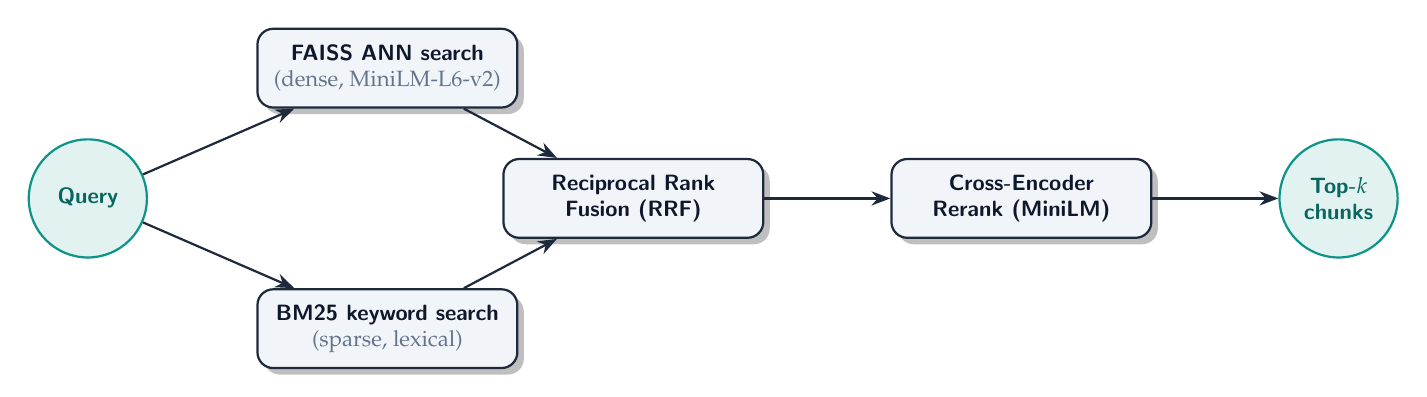
\begin{tikzpicture}[
    node distance=8mm and 14mm,
    stage/.style={draw=navylight, thick, rounded corners=2mm, fill=palegray,
                minimum width=3.3cm, minimum height=1.0cm, align=center,
                font=\sffamily\footnotesize\bfseries\color{navy}, drop shadow},
    query/.style={draw=teal, thick, circle, fill=teal!12, minimum size=1.5cm,
                font=\sffamily\footnotesize\bfseries\color{tealdark}, align=center},
    arr/.style={-{Stealth[length=2.4mm]}, thick, navylight}
]
\node[query] (q) {Query};
\node[stage, above right=6mm and 16mm of q] (faiss) {FAISS ANN search\\ \footnotesize\normalfont\color{softgray}(dense, MiniLM-L6-v2)};
\node[stage, below right=6mm and 16mm of q] (bm25) {BM25 keyword search\\ \footnotesize\normalfont\color{softgray}(sparse, lexical)};
\node[stage, right=45mm of q] (fuse) {Reciprocal Rank\\Fusion (RRF)};
\node[stage, right=16mm of fuse] (rerank) {Cross-Encoder\\Rerank (MiniLM)};
\node[query, right=16mm of rerank] (topk) {Top-$k$\\chunks};

\draw[arr] (q) -- (faiss);
\draw[arr] (q) -- (bm25);
\draw[arr] (faiss) -- (fuse);
\draw[arr] (bm25) -- (fuse);
\draw[arr] (fuse) -- (rerank);
\draw[arr] (rerank) -- (topk);
\end{tikzpicture}
\caption{The hybrid retrieval pipeline: two independent candidate lists (dense + sparse) are fused by rank, then reranked by a cross-encoder that actually reads query and chunk together.}
\label{fig:retrieval}
\end{figure}

\subsection{\texttt{retriver.py} --- Corpus Discovery}

Walks the \texttt{data/} directory recursively, skipping VCS/build noise
(\texttt{.git}, \texttt{\_\_pycache\_\_}, \texttt{venv}, \texttt{node\_modules},
\texttt{dist}, \texttt{build}), and reads every remaining file into memory as
\texttt{(Path, content)} pairs. This is the corpus boundary every other file
in this project respects.

\begin{pycode}[retriver.py]
from pathlib import Path

ignored_dirs = {
    ".git", "__pycache__", ".venv", "venv",
    "node_modules", "dist", "build"
}

def discover_files(p):
    files = []
    for item in p.iterdir():
        if item.is_dir():
            if item.name not in ignored_dirs:
                files.extend(discover_files(item))
        elif item.is_file():
            files.append(item)
    return files

p = Path("data")
files_name = discover_files(p)

text_files = []
for file in files_name:
    with open(str(file), "r", encoding="utf-8") as f:
        content = f.read()
        text_files.append((file, content))
\end{pycode}

\subsection{\texttt{chunking.py} --- Fixed-Window Chunking}

Splits every file's content into 400-character windows. Simple by design --
chunk identity (its index into the global \texttt{chunks} list) is the
common key every downstream index (FAISS, BM25) refers back to.

\begin{pycode}[chunking.py]
from retriver import text_files

chunks = []
for file, content in text_files:
    for i in range(0, len(content), 400):
        chunk = content[i:i+400]
        chunks.append((file, chunk))
\end{pycode}

\subsection{\texttt{embeddings.py} --- Dense Vectors}

Encodes every chunk with \texttt{sentence-transformers}' \texttt{all-MiniLM-L6-v2}
(384-dimensional) at import time, and exposes \texttt{query\_embedding()} for
encoding a query the same way at request time.

\begin{pycode}[embeddings.py]
from sentence_transformers import SentenceTransformer
from chunking import chunks

model = SentenceTransformer('all-MiniLM-L6-v2')
embeddings_list_whole = []
embeddings_list = []
for file, content in chunks:
    embeddings = model.encode(content)
    embeddings_list.append(embeddings)
    embeddings_list_whole.append((file, content, embeddings))

def query_embedding(query):
    query_vector = model.encode([query]).astype('float32')
    return query_vector
\end{pycode}

\subsection{\texttt{Faiss\_Searach.py} --- Dense Nearest-Neighbour Index}

Builds a flat L2 FAISS index (\texttt{IndexFlatL2}, dimension 384) over every
chunk embedding, and exposes \texttt{query\_indices()} for top-$k$ nearest
neighbour search.

\begin{pycode}[Faiss_Searach.py]
import faiss
import numpy as np
from embeddings import embeddings_list

embeddings_array = np.array(embeddings_list, dtype='float32')
dimension = 384
index = faiss.IndexFlatL2(dimension)
index.add(embeddings_array)

def query_indices(query_vector, top_k=3):
    scores, indices = index.search(query_vector, top_k)
    return scores, indices
\end{pycode}

\subsection{\texttt{Hybrid\_Search.py} --- Sparse Search \& Reranking}

Builds a \texttt{rank\_bm25} \texttt{BM25Okapi} index over lower-cased,
whitespace-tokenized chunks, and loads a
\texttt{cross-encoder/ms-marco-MiniLM-L-6-v2} model that scores
\texttt{(query, chunk)} pairs jointly -- the step that actually separates a
truly relevant chunk from one that merely shares vocabulary with the query.

\begin{pycode}[Hybrid_Search.py]
from chunking import chunks
from rank_bm25 import BM25Okapi
from sentence_transformers import CrossEncoder

tokenized_chunks = [chunk[1].lower().split() for chunk in chunks]
bm25 = BM25Okapi(tokenized_chunks)
cross_encoder = CrossEncoder("cross-encoder/ms-marco-MiniLM-L-6-v2")

def query_bm25(query, top_k=5):
    tokenized_query = query.lower().split()
    scores = bm25.get_scores(tokenized_query)
    top_indices = scores.argsort()[-top_k:][::-1]
    return top_indices

def rerank(query, ranked_chunks, top_k=5):
    pairs = [[query, chunks[chunk_id][1]] for chunk_id, rrf_score in ranked_chunks]
    scores = cross_encoder.predict(pairs)
    reranked = sorted(zip(ranked_chunks, scores), key=lambda x: x[1], reverse=True)
    return [(int(chunk_id), float(score))
            for ((chunk_id, rrf_score), score) in reranked[:top_k]]
\end{pycode}

\subsection{\texttt{llm\_calling.py} --- Orchestration \& the Shared Pipeline}

This is where the pieces above are fused together, and it is the single
place both the standalone \texttt{the\_call()} entry point \emph{and} the MCP
server's \texttt{search\_documents} tool draw from -- so the Reciprocal Rank
Fusion logic exists exactly once in the entire codebase.

\begin{pycode}[llm_calling.py -- shared retrieval core]
def _rrf_fuse(bm25_indices, faiss_indices, k=60):
    rrf_scores = {}
    for rank, chunk_id in enumerate(bm25_indices, start=1):
        rrf_scores[chunk_id] = rrf_scores.get(chunk_id, 0) + 1 / (k + rank)
    for rank, chunk_id in enumerate(faiss_indices, start=1):
        rrf_scores[chunk_id] = rrf_scores.get(chunk_id, 0) + 1 / (k + rank)
    return sorted(rrf_scores.items(), key=lambda x: x[1], reverse=True)

def retrieve_ranked_chunks(query, top_k=10, rerank_top_k=5):
    query_vector = query_embedding(query)
    scores, faiss_indices = query_indices(query_vector, top_k=top_k)
    faiss_indices = faiss_indices[0]
    bm25_indices = query_bm25(query, top_k=top_k)
    ranked_chunks = _rrf_fuse(bm25_indices, faiss_indices)
    if not ranked_chunks:
        return []
    return rerank(query, ranked_chunks, top_k=rerank_top_k)

def the_call(query):
    reranked_chunks = retrieve_ranked_chunks(query, top_k=10, rerank_top_k=5)
    if not reranked_chunks:
        return ""
    top_chunks = [chunks[chunk_id] for chunk_id, score in reranked_chunks[:2]]
    return "\n\n".join(chunk[1] for chunk in top_chunks)

def search_documents_structured(query, top_k=5):
    if not isinstance(query, str) or not query.strip():
        return {"success": False, "results": [], "error": "query must be a non-empty string"}
    try:
        reranked_chunks = retrieve_ranked_chunks(query, top_k=max(10, top_k * 2), rerank_top_k=top_k)
    except Exception as e:
        return {"success": False, "results": [], "error": f"retrieval failed: {e}"}
    if not reranked_chunks:
        return {"success": False, "results": [], "error": "No relevant documents found"}
    results = []
    for chunk_id, score in reranked_chunks:
        file_path, chunk_text = chunks[chunk_id]
        results.append({"file": str(file_path), "text": chunk_text, "score": float(score)})
    return {"success": True, "results": results, "error": None}
\end{pycode}

\begin{successbox}[No duplicated algorithms]
\texttt{retrieve\_ranked\_chunks()} is the \emph{only} place the
BM25/FAISS/RRF/cross-encoder orchestration exists. \texttt{the\_call()} (the
original entry point) and \texttt{search\_documents\_structured()} (the MCP
tool's backing function) both call it -- they differ only in how they shape
the \emph{output} (one concatenated string vs.\ a structured, per-chunk list
with file and score).
\end{successbox}



\clearpage
\section{The LangGraph Multi-Agent System}
\label{sec:langgraph}

\texttt{Multi\_Agent\_System.py} is the executable heart of the project: it
defines the shared state, every node function, and wires them into a
compiled LangGraph \texttt{StateGraph}.

\subsection{State Schema}

\begin{pycode}[Multi_Agent_System.py -- AgentState]
class AgentState(TypedDict):
    messages: list
    query: str
    current_query: str
    plan: list                 # append-only trace of search goals tried
    retrieved_chunks: list     # text the Critic/Synthesizer read
    tool_results: list         # {tool_name, args, success, error} per call
    critic_result: dict
    iteration_count: int
    final_answer: str
\end{pycode}

\begin{tabularx}{\textwidth}{@{}l l X@{}}
\toprule
\rowcolor{navylight}
\textcolor{white}{\textbf{Field}} & \textcolor{white}{\textbf{Type}} & \textcolor{white}{\textbf{Purpose}} \\
\midrule
\texttt{query} & \texttt{str} & The original user question; never overwritten. \\
\texttt{current\_query} & \texttt{str} & The Planner's latest refined search query. \\
\texttt{plan} & \texttt{list} & Every \texttt{current\_query} tried so far, in order. \\
\texttt{retrieved\_chunks} & \texttt{list} & Raw evidence text the Critic/Synthesizer join and read. \\
\texttt{tool\_results} & \texttt{list} & Structured record of every tool call: name, args, success, error. \\
\texttt{critic\_result} & \texttt{dict} & \texttt{\{verdict, reasoning, missing\_info, suggested\_tool?\}}. \\
\texttt{iteration\_count} & \texttt{int} & Retry counter; the Router stops looping at 3. \\
\texttt{final\_answer} & \texttt{str} & The Synthesizer's grounded, cited answer. \\
\bottomrule
\end{tabularx}

\vspace{6pt}
\begin{infobox}[Why both \texttt{retrieved\_chunks} and \texttt{tool\_results}?]
\texttt{retrieved\_chunks} decides \emph{what the LLM reads}; \texttt{tool\_results}
decides \emph{what the Critic reasons about}. Keeping them separate means the
Critic can tell the Tool Agent "try \texttt{search\_code} instead" without the
Synthesizer's prompt needing to change at all.
\end{infobox}

\subsection{Node: \texttt{planner}}
Turns the raw question (or, on a retry, the question plus the Critic's
\texttt{reasoning}/\texttt{missing\_info}) into a keyword-dense search query
via \texttt{PLANNER\_SYSTEM\_PROMPT}.

\begin{pycode}[Multi_Agent_System.py -- planner]
def planner(state: AgentState):
    iteration = state.get("iteration_count", 0)
    user_query = state.get("query", "")
    critic_feedback = state.get("critic_result", {})

    if iteration > 0 and critic_feedback:
        prompt_content = (
            f"Original Query: {user_query}\n"
            f"Previous attempt was insufficient: {critic_feedback.get('reasoning', '')}\n"
            f"Missing context: {critic_feedback.get('missing_info', '')}\n"
            f"Formulate a refined, targeted search query."
        )
    else:
        prompt_content = f"Target technical query: {user_query}"

    messages = [SystemMessage(content=PLANNER_SYSTEM_PROMPT), HumanMessage(content=prompt_content)]
    response = llm.invoke(messages)
    return {"current_query": response.content.strip(), "iteration_count": iteration + 1}
\end{pycode}

\subsection{Node: \texttt{tool\_agent} --- the Tool Agent}
\label{sec:toolagent}

This node replaced the original, hardcoded \texttt{retriever} node. It is
covered in full detail in Section~\ref{sec:toolagentdeep}; in outline, it:

\begin{enumerate}
\item Converts the MCP server's live tool list into OpenAI-style function
      schemas (\texttt{get\_llm\_tool\_schemas()}).
\item If the Critic left a \texttt{suggested\_tool} from the previous
      iteration, calls that tool directly (deterministic override).
\item Otherwise binds the schemas to the LLM (\texttt{llm.bind\_tools(...)})
      and lets the model choose a tool call.
\item If the model returns no tool call at all, falls back to a plain
      \texttt{search\_documents} call -- the original Step~4 behaviour.
\item Dispatches every resulting tool call through
      \texttt{mcp\_client.call\_tool\_json(name, args)} and folds the
      results into \texttt{tool\_results} and \texttt{retrieved\_chunks}.
\end{enumerate}

\subsection{Node: \texttt{critic\_agent}}
Judges whether the retrieved evidence is sufficient, now with visibility
into \emph{which tool} produced it:

\begin{pycode}[Multi_Agent_System.py -- critic_agent]
def critic_agent(state: AgentState):
    chunks_text = "\n\n".join(state.get("retrieved_chunks", []))
    tool_results = state.get("tool_results", [])
    tool_usage_summary = "\n".join(
        f"- {r.get('tool_name')} (success={r.get('success')})"
        + (f" error={r.get('error')}" if not r.get("success") and r.get("error") else "")
        for r in tool_results
    ) or "No tool calls recorded."

    prompt_content = (
        f"Original User Question: {state.get('query', '')}\n\n"
        f"Tool calls made so far:\n{tool_usage_summary}\n\n"
        f"Retrieved Evidence Chunks:\n{chunks_text}"
    )
    messages = [SystemMessage(content=CRITIC_SYSTEM_PROMPT), HumanMessage(content=prompt_content)]
    response = llm.invoke(messages)
    try:
        parsed_result = json.loads(response.content.strip())
    except Exception:
        parsed_result = {"verdict": "FAIL", "reasoning": "Output parsing failed.",
                          "missing_info": "Unable to verify context validity."}
    return {"critic_result": parsed_result}
\end{pycode}

\subsection{Node: \texttt{router} (conditional edge)}
A pure function, not an LLM call -- three lines of logic decide the entire
retry policy:

\begin{pycode}[Multi_Agent_System.py -- router]
def router(state: AgentState):
    MAX_RETRIES = 3
    verdict = state.get("critic_result", {}).get("verdict", "FAIL")
    if verdict == "PASS":
        return "Synthesizer"
    if state.get("iteration_count", 0) < MAX_RETRIES:
        return "planner"
    return "Synthesizer"
\end{pycode}

\subsection{Node: \texttt{Synthesizer}}
Produces the final, evidence-grounded answer via \texttt{SYNTHESIZER\_SYSTEM\_PROMPT}
-- a nine-rule prompt (Section~\ref{sec:prompts}) that forbids fabricating
file names, requires a \textit{Root Cause / Evidence / Fix} structure, and
requires inline \texttt{[filename]} citations.

\begin{pycode}[Multi_Agent_System.py -- Synthesizer]
def Synthesizer(state: AgentState):
    chunks_text = "\n\n".join(state.get("retrieved_chunks", []))
    prompt_content = f"User Inquiry: {state.get('query', '')}\n\nRetrieved Context:\n{chunks_text}"
    messages = [SystemMessage(content=SYNTHESIZER_SYSTEM_PROMPT), HumanMessage(content=prompt_content)]
    response = llm.invoke(messages)
    return {"final_answer": response.content}
\end{pycode}

\subsection{Graph Assembly}

\begin{pycode}[Multi_Agent_System.py -- graph wiring]
graph_builder = StateGraph(AgentState)
graph_builder.add_node("planner", planner)
graph_builder.add_node("tool_agent", tool_agent)
graph_builder.add_node("critic_agent", critic_agent)
graph_builder.add_node("Synthesizer", Synthesizer)

graph_builder.add_edge(START, "planner")
graph_builder.add_edge("planner", "tool_agent")
graph_builder.add_edge("tool_agent", "critic_agent")
graph_builder.add_conditional_edges(
    "critic_agent", router, {"planner": "planner", "Synthesizer": "Synthesizer"}
)
graph_builder.add_edge("Synthesizer", END)
graph = graph_builder.compile()
\end{pycode}

\clearpage
\subsection{The System Prompts}
\label{sec:prompts}

Every LLM call in the graph is governed by one of four prompts defined in
\texttt{Agent\_prompts.py}. None of them touch retrieval mechanics directly
-- they only shape reasoning and output format.

\begin{tabularx}{\textwidth}{@{}l X@{}}
\toprule
\rowcolor{navylight}
\textcolor{white}{\textbf{Prompt}} & \textcolor{white}{\textbf{Role}} \\
\midrule
\texttt{PLANNER\_SYSTEM\_PROMPT} & Strips conversational filler; outputs only a keyword-dense search query. \\
\texttt{TOOL\_AGENT\_SYSTEM\_PROMPT} & Describes all three MCP tools and when to prefer each; instructs the model never to invent a \texttt{retrieve\_file} path. \\
\texttt{CRITIC\_SYSTEM\_PROMPT} & Judges sufficiency \& hallucination risk; may emit \texttt{suggested\_tool} on FAIL. \\
\texttt{SYNTHESIZER\_SYSTEM\_PROMPT} & Nine operational rules: strict evidence grounding, root-cause-first structure, inline citations, no fabrication. \\
\bottomrule
\end{tabularx}

\begin{pycode}[Agent_prompts.py -- CRITIC_SYSTEM_PROMPT (response schema excerpt)]
RESPONSE FORMAT:
You must respond ONLY with a raw, valid JSON object matching this exact structure:
{
  "verdict": "PASS" | "FAIL",
  "reasoning": "<Concise explanation of whether the context is sufficient>",
  "missing_info": "<Specific missing configuration, line, or file if FAIL>",
  "suggested_tool": "<search_documents | search_code | retrieve_file -- ONLY
                      when verdict is FAIL and a different tool would help>"
}
\end{pycode}



\section{The MCP Layer: Server \& Client}
\label{sec:mcp}

Everything described so far -- the retrieval pipeline and the LangGraph
agent -- existed before this layer was added. The Model Context Protocol
(MCP) layer wraps the retrieval pipeline behind a real, standalone,
independently-executable server process, and gives the LangGraph agent a
\emph{client} that speaks the official MCP wire protocol to it over
\texttt{stdio}. No retrieval algorithm was rewritten; MCP only changes
\emph{how} the agent reaches the existing code.

\begin{infobox}{Why a protocol instead of a function call?}
A plain Python import (\texttt{from llm\_calling import the\_call}) would
have been far simpler -- and would have been the wrong deliverable. MCP
tools are described by machine-readable JSON Schemas that the agent
discovers \emph{at runtime}, over a real subprocess boundary, using the
official \texttt{mcp} SDK. That is what makes tool selection dynamic
(Section~\ref{sec:toolagent}) instead of hard-coded.
\end{infobox}

\subsection{Process Architecture}

Two independent OS processes communicate over a pair of anonymous pipes
(\texttt{stdin}/\texttt{stdout}), framed as JSON-RPC 2.0 messages. Figure
\ref{fig:mcp} shows the full picture.

\begin{figure}[H]
\centering
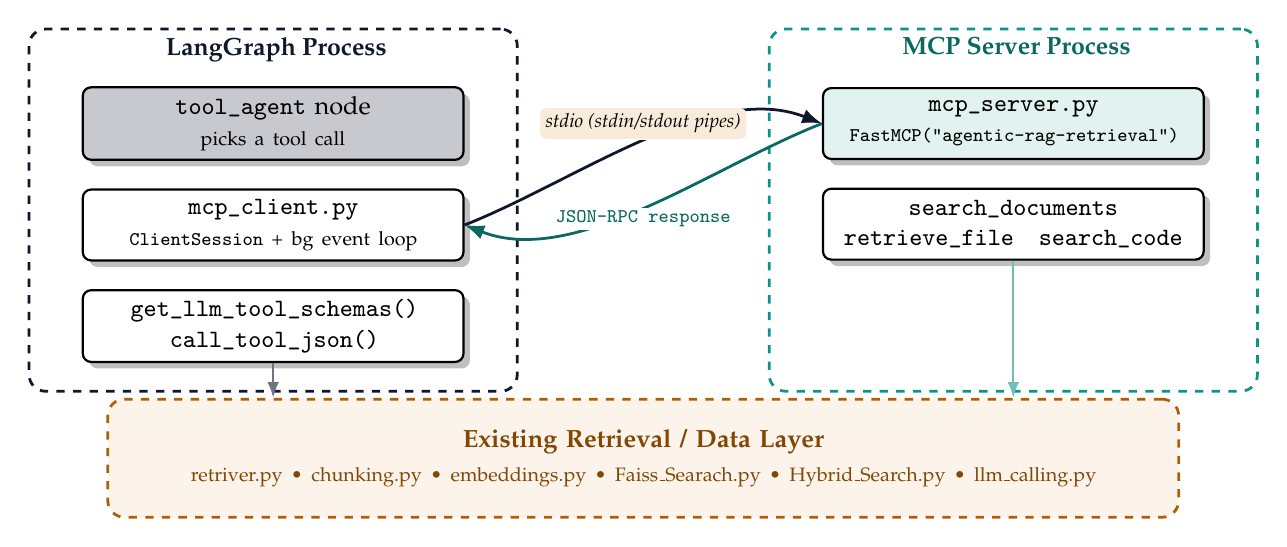
\begin{tikzpicture}[
    node distance=0.9cm and 1.6cm,
    box/.style={draw, rounded corners=3pt, minimum height=0.9cm, font=\small,
                fill=white, drop shadow, line width=0.8pt},
    proc/.style={draw, rounded corners=6pt, dashed, inner sep=10pt, line width=1pt},
    lbl/.style={font=\scriptsize\ttfamily, fill=white, inner sep=1pt}
]
    \node[proc, draw=navy, minimum width=6.2cm, minimum height=4.6cm] (langgraph) at (0,-0.2) {};
    \node[font=\bfseries\small\color{navy}, anchor=north] at (langgraph.north) {\vphantom{Xy} LangGraph Process};

    \node[box, fill=navylight!25, text width=4.6cm, align=center] (toolagent) at (0,0.9) {\texttt{tool\_agent} node\\\scriptsize picks a tool call};
    \node[box, fill=white, text width=4.6cm, align=center, below=0.35cm of toolagent] (client) {\texttt{mcp\_client.py}\\\scriptsize \texttt{ClientSession} + bg event loop};
    \node[box, fill=white, text width=4.6cm, align=center, below=0.35cm of client] (schemas) {\texttt{get\_llm\_tool\_schemas()}\\\texttt{call\_tool\_json()}};

    \node[proc, draw=teal, minimum width=6.2cm, minimum height=4.6cm] (server) at (9.4,-0.2) {};
    \node[font=\bfseries\small\color{teal!70!black}, anchor=north] at (server.north) {\vphantom{Xy} MCP Server Process};

    \node[box, fill=teal!12, text width=4.6cm, align=center] (fastmcp) at (9.4,0.9) {\texttt{mcp\_server.py}\\\scriptsize \texttt{FastMCP("agentic-rag-retrieval")}};
    \node[box, fill=white, text width=4.6cm, align=center, below=0.35cm of fastmcp] (tools) {\texttt{search\_documents}\\\texttt{retrieve\_file}\quad\texttt{search\_code}};

    \draw[-{Latex[length=2.5mm]}, line width=1pt, navy]
        (client.east) .. controls +(1.4,0.55) and +(-1.4,0.55) .. node[lbl, above, midway]{JSON-RPC request} (fastmcp.west);
    \draw[-{Latex[length=2.5mm]}, line width=1pt, teal!70!black]
        (fastmcp.west) .. controls +(-1.4,-0.55) and +(1.4,-0.55) .. node[lbl, below, midway]{JSON-RPC response} (client.east);
    \node[font=\scriptsize\itshape, fill=amber!15, rounded corners=2pt, inner sep=2pt] at (4.7,0.9) {stdio (stdin/stdout pipes)};

    \node[proc, draw=amber!80!black, minimum width=13.6cm, minimum height=1.5cm, fill=amber!8] (data) at (4.7,-3.35) {};
    \node[font=\bfseries\small\color{amber!60!black}, align=center, text width=12.5cm] at (data.center) {Existing Retrieval / Data Layer\\[1pt] \scriptsize\normalfont retriver.py \textbullet\ chunking.py \textbullet\ embeddings.py \textbullet\ Faiss\_Searach.py \textbullet\ Hybrid\_Search.py \textbullet\ llm\_calling.py};

    \draw[-{Latex[length=2mm]}, line width=0.8pt, navy!60] (schemas.south) -- ++(0,-0.25) -| (data.north -| toolagent);
    \draw[-{Latex[length=2mm]}, line width=0.8pt, teal!60] (tools.south) -- (tools.south |- data.north);
\end{tikzpicture}
\caption{The MCP server and the LangGraph process are separate OS processes. The client launches the server as a subprocess via \texttt{StdioServerParameters} and speaks framed JSON-RPC 2.0 over its stdin/stdout. Only the server process imports the retrieval modules directly.}
\label{fig:mcp}
\end{figure}

\begin{warnbox}{This is a real subprocess, not a fake protocol}
\texttt{mcp\_server.py} is executed by \texttt{sys.executable mcp\_server.py} as
a genuinely separate OS process (verifiable with \texttt{ps} while a query
runs). The LangGraph process never imports \texttt{mcp\_server.py}. Every
tool call is round-tripped through the official \texttt{mcp} Python SDK's
\texttt{ClientSession}, serialized to JSON-RPC, written to a pipe, and
parsed back on the other side -- exactly like a network-based MCP server,
except the transport is \texttt{stdio} instead of HTTP/SSE.
\end{warnbox}

\subsection{\texttt{mcp\_server.py} -- the standalone server}

The server is a single file that can be run on its own
(\texttt{python mcp\_server.py}) with no LangGraph or agent code loaded at
all. It builds a \texttt{FastMCP} instance and registers three tools with
the \texttt{@mcp.tool()} decorator; FastMCP derives each tool's JSON Schema
automatically from the function's type hints and docstring.

\begin{pycode}[mcp_server.py -- server bootstrap and search_documents]
PROJECT_ROOT = Path(__file__).resolve().parent
sys.path.insert(0, str(PROJECT_ROOT))

from mcp.server.fastmcp import FastMCP
from llm_calling import search_documents_structured

DATA_DIR = (PROJECT_ROOT / "data").resolve()
mcp = FastMCP("agentic-rag-retrieval")

@mcp.tool()
def search_documents(query: str, top_k: int = 5) -> dict:
    """Search the indexed document corpus using BM25 + FAISS + RRF
    + cross-encoder reranking. Returns the most relevant chunks."""
    if not isinstance(query, str) or not query.strip():
        return {"success": False, "results": [], "error": "query must be a non-empty string"}
    try:
        top_k = int(top_k)
    except (TypeError, ValueError):
        return {"success": False, "results": [], "error": "top_k must be an integer"}
    if top_k <= 0:
        return {"success": False, "results": [], "error": "top_k must be a positive integer"}
    try:
        return search_documents_structured(query, top_k=top_k)
    except Exception as e:
        return {"success": False, "results": [], "error": f"unexpected error: {e}"}

if __name__ == "__main__":
    mcp.run(transport="stdio")
\end{pycode}

Notice that \texttt{search\_documents} never re-implements BM25, FAISS,
RRF or reranking -- it calls \texttt{search\_documents\_structured()},
which lives in the pre-existing \texttt{llm\_calling.py} and simply wraps
the pre-existing \texttt{retrieve\_ranked\_chunks()} pipeline in a
structured, JSON-serializable \texttt{\{success, results, error\}} shape.
Every failure path (empty query, bad \texttt{top\_k}, retrieval exception,
zero results) returns a well-formed dict instead of raising -- the tool
boundary never lets a raw Python exception escape to the JSON-RPC layer.

\subsection{Corpus-boundary enforcement: \texttt{retrieve\_file}}

\texttt{retrieve\_file} lets the agent open a specific chunk's source file
in full. Because the argument is an LLM-supplied string, it must never be
trusted as a raw filesystem path -- the tool resolves it strictly inside
\texttt{data/} and rejects anything that would escape it.

\begin{pycode}[mcp_server.py -- path-restricted file access]
def _resolve_within_data(relative_path: str) -> Path:
    normalized = relative_path.replace("\\", "/")
    if normalized == "data" or normalized.startswith("data/"):
        normalized = normalized[len("data"):].lstrip("/")
    candidate = (DATA_DIR / normalized).resolve()
    if candidate != DATA_DIR and DATA_DIR not in candidate.parents:
        raise ValueError("path escapes the data/ corpus directory")
    return candidate

@mcp.tool()
def retrieve_file(path: str) -> dict:
    """Read the full contents of one file inside the data/ corpus."""
    if not isinstance(path, str) or not path.strip():
        return {"success": False, "path": path, "content": None,
                 "error": "path must be a non-empty string"}
    try:
        resolved = _resolve_within_data(path)
    except ValueError as e:
        return {"success": False, "path": path, "content": None, "error": str(e)}
    if not resolved.exists() or not resolved.is_file():
        return {"success": False, "path": path, "content": None,
                 "error": f"file not found: {path}"}
    content = resolved.read_text(encoding="utf-8", errors="replace")
    return {"success": True, "path": path, "content": content, "error": None}
\end{pycode}

\begin{dangerbox}{Path traversal is blocked by resolution, not string matching}
The guard resolves the candidate path with \texttt{Path.resolve()} (which
collapses \texttt{..} segments and symlinks) and then checks real
directory containment via \texttt{.parents}, not a naive
\texttt{str.startswith("data/")} check. A payload such as
\texttt{"../../etc/passwd"} or \texttt{"..\textbackslash..\textbackslash Windows\textbackslash win.ini"}
resolves outside \texttt{DATA\_DIR} and is rejected with
\texttt{"path escapes the data/ corpus directory"} before any file I/O is
attempted. Verified directly in \texttt{test\_mcp\_integration.py}.
\end{dangerbox}

\subsection{MCP Tool Specification}

\begin{table}[H]
\centering
\small
\begin{tabularx}{\textwidth}{@{}l X X@{}}
\toprule
\rowcolor{navylight}
\textcolor{white}{\textbf{Tool}} & \textcolor{white}{\textbf{Arguments}} & \textcolor{white}{\textbf{Returns}} \\
\midrule
\texttt{search\_documents} & \texttt{query: str}, \texttt{top\_k: int = 5} &
\texttt{\{success, results: [\{file, text, score\}], error\}} -- hybrid BM25+FAISS+RRF+cross-encoder search over the full corpus. \\
\addlinespace
\texttt{retrieve\_file} & \texttt{path: str} &
\texttt{\{success, path, content, error\}} -- full text of one file, resolved strictly inside \texttt{data/}. \\
\addlinespace
\texttt{search\_code} & \texttt{query: str}, \texttt{top\_k: int = 5} &
\texttt{\{success, results: [\{file, text\}], error\}} -- BM25 search filtered to source/config file extensions only. \\
\bottomrule
\end{tabularx}
\caption{All three tools are pure functions of their arguments: no shared mutable state, no side effects outside reading \texttt{data/}.}
\end{table}

\subsection{\texttt{mcp\_client.py} -- launching and talking to the server}

The client is the only file that knows the server is a subprocess. It
launches \texttt{mcp\_server.py} with \texttt{StdioServerParameters},
pinning \texttt{cwd} to the project root so the server's own relative
\texttt{Path("data")} lookups resolve correctly regardless of where the
LangGraph process itself was started from.

\begin{pycode}[mcp_client.py -- subprocess launch]
async def _connect(self):
    params = StdioServerParameters(
        command=sys.executable,
        args=[str(PROJECT_ROOT / "mcp_server.py")],
        cwd=str(PROJECT_ROOT),
    )
    self._stdio_ctx = stdio_client(params)
    read, write = await self._stdio_ctx.__aenter__()
    self._session = ClientSession(read, write)
    await self._session.__aenter__()
    await self._session.initialize()
\end{pycode}

Because LangGraph nodes are synchronous functions but the MCP SDK is
\texttt{async}, \texttt{mcp\_client.py} runs one long-lived
\texttt{asyncio} event loop on a background thread and bridges every call
across it with \texttt{run\_coroutine\_threadsafe}. The public entry point,
\texttt{call\_tool\_json()}, is what the Tool Agent node actually calls --
it is dynamic dispatch by tool \emph{name}, never a static
\texttt{if/elif} chain:

\begin{pycode}[mcp_client.py -- dynamic dispatch entry point]
def call_tool_json(name: str, arguments: dict) -> dict:
    _guard_destructive_tool(name)          # Section 6.4 hook
    try:
        result = get_manager().call_tool(name, arguments)
    except MCPServerError as e:
        return {"success": False, "results": [], "error": str(e)}
    text = _extract_text(result)
    return _validate_tool_response(name, text)   # Pydantic boundary check
\end{pycode}

Whatever the agent asks for -- \texttt{search\_documents},
\texttt{retrieve\_file}, or \texttt{search\_code} -- flows through this
exact same function. Adding a fourth tool to \texttt{mcp\_server.py}
requires \emph{zero} changes here: \texttt{get\_llm\_tool\_schemas()}
(Section~\ref{sec:toolagent}) would simply discover it at the next
\texttt{list\_tools()} call.


\section{The Tool Agent Layer: Autonomous Selection, State \& Resilience}
\label{sec:toolagentdeep}

The Step~4 baseline gave the agent \emph{a} tool call, but the choice of
tool was still effectively deterministic. This layer turns
\texttt{tool\_agent} into something that genuinely decides, degrades
gracefully when the server misbehaves, and is structurally ready for a
human-in-the-loop approval gate. It rests on four pillars.

\subsection{Pillar 1 -- Autonomous Tool Selection}

Every MCP tool schema is discovered live, not hand-written twice. The
same JSON Schema FastMCP derived for the wire protocol is reshaped into
the OpenAI function-calling format and handed straight to
\texttt{llm.bind\_tools(...)}:

\begin{pycode}[mcp_client.py -- schema translation]
def get_llm_tool_schemas():
    schemas = []
    for tool in list_available_tools():
        schemas.append({
            "type": "function",
            "function": {
                "name": tool.name,
                "description": tool.description or "",
                "parameters": tool.inputSchema or {"type": "object", "properties": {}},
            },
        })
    return schemas
\end{pycode}

\begin{pycode}[Multi_Agent_System.py -- binding and dynamic dispatch]
tool_schemas = get_llm_tool_schemas()
bound_llm = llm.bind_tools(tool_schemas)
response = bound_llm.invoke(messages)          # model decides
tool_calls = getattr(response, "tool_calls", None) or []

for call in tool_calls:
    result = call_tool_json(call["name"], call["args"])   # dynamic, by name
\end{pycode}

There is no \texttt{if tool == "search\_documents": ... elif tool ==
"retrieve\_file": ...} anywhere in the agent. \texttt{TOOL\_AGENT\_SYSTEM\_PROMPT}
(Section~\ref{sec:prompts}) tells the model \emph{when} each tool is
appropriate; the model tells the graph \emph{which one} to call for this
particular question, and \texttt{call\_tool\_json} dispatches purely on
the returned tool name. A registered fourth or fifth tool would be picked
up automatically the next time \texttt{get\_llm\_tool\_schemas()} runs --
nothing in \texttt{Multi\_Agent\_System.py} would need to change.

\subsection{Pillar 2 -- State Alignment}

\texttt{AgentState} grew two fields to support this: \texttt{plan} (a
running log of every search query the Planner has issued, so the Tool
Agent can see what's already been tried) and \texttt{tool\_results} (a
list of structured records -- one per tool call -- decoupled from the raw
evidence text):

\begin{table}[H]
\centering
\small
\begin{tabularx}{\textwidth}{@{}l l X@{}}
\toprule
\rowcolor{navylight}
\textcolor{white}{\textbf{Field}} & \textcolor{white}{\textbf{Type}} & \textcolor{white}{\textbf{Role}} \\
\midrule
\texttt{plan} & \texttt{list[str]} & Every query the Planner has issued so far this run. \\
\texttt{tool\_results} & \texttt{list[dict]} & \texttt{\{tool\_name, args, success, error\}} per call -- lets the Critic reason about \emph{which tool} produced (or failed to produce) evidence. \\
\texttt{retrieved\_chunks} & \texttt{list[str]} & Unchanged from Step~4 -- raw evidence text handed to the Critic/Synthesizer, kept separate from call metadata. \\
\bottomrule
\end{tabularx}
\caption{Only two fields were added; every other field in \texttt{AgentState} is unchanged from the original graph.}
\end{table}

Separating \texttt{tool\_results} from \texttt{retrieved\_chunks} is what
lets \texttt{critic\_agent} say ``\texttt{search\_code} failed, try
\texttt{search\_documents} instead'' via the new \texttt{suggested\_tool}
field, without needing to parse evidence strings to guess what happened.

\subsection{Pillar 3 -- Graceful Degradation \& Schema Fallbacks}

Two independent safety nets sit at the client/server boundary.

\textbf{Pydantic validation.} Every response coming back over
\texttt{stdio} is parsed through a permissive Pydantic model before the
agent ever sees it. A truncated pipe write, a malformed JSON fragment, or
a tool that forgot to include \texttt{success} all collapse to the same
predictable shape instead of raising deep inside the graph:

\begin{pycode}[mcp_client.py -- response validation]
class _MCPToolResponse(BaseModel):
    model_config = ConfigDict(extra="allow")
    success: bool
    error: Optional[str] = None

def _validate_tool_response(name: str, raw_text: str) -> dict:
    try:
        data = json.loads(raw_text)
        validated = _MCPToolResponse.model_validate(data)
        return {**data, "success": validated.success}
    except (json.JSONDecodeError, ValidationError) as e:
        return {"success": False, "results": [],
                 "error": f"malformed response from '{name}': {e}"}
\end{pycode}

\textbf{Automatic respawn-and-retry.} If the subprocess connection itself
dies mid-call (broken pipe, crashed server, closed stdio), the manager
tears down the dead session, launches a brand-new server subprocess,
re-initializes the MCP handshake, and retries the \emph{same} call
\textbf{exactly once} before giving up:

\begin{pycode}[mcp_client.py -- respawn-once-then-fail]
def _run(self, coro_fn, timeout=60, _respawned=False):
    try:
        self._ensure_started()
        future = asyncio.run_coroutine_threadsafe(coro_fn(), self._loop)
        return future.result(timeout=timeout)
    except Exception as e:
        self._reset_connection()
        if not _respawned:
            return self._run(coro_fn, timeout=timeout, _respawned=True)
        raise MCPServerError(f"MCP server unavailable after respawn: {e}")
\end{pycode}

\begin{successbox}{Verified with a real subprocess kill, not a mock}
\texttt{test\_mcp\_integration.py} exercises this exact code path by
monkeypatching the live session's \texttt{call\_tool} to raise
\texttt{ConnectionResetError} on its first invocation only, then
confirming the \emph{unmodified production} \texttt{\_reset\_connection()}
logic spins up a genuinely new subprocess and the retry succeeds. If the
respawned server also fails, \texttt{MCPServerError} propagates up to
\texttt{tool\_agent}, which converts it into a well-formed FAIL verdict
(\texttt{\_mcp\_unavailable\_result}) rather than crashing the graph.
\end{successbox}

\subsection{Pillar 4 -- Preparation for Step 5 (Human-in-the-Loop Gate)}

Every tool is classified by safety, and the classification is enforced
\emph{before} any JSON-RPC call leaves the client process:

\begin{pycode}[mcp_client.py -- tool safety classification and pre-hook]
READ_ONLY_TOOLS = {"search_documents", "retrieve_file", "search_code"}
DESTRUCTIVE_TOOLS = {"create_issue", "modify_file", "run_sql_mutation"}

def _guard_destructive_tool(name: str):
    if name not in DESTRUCTIVE_TOOLS:
        return                                   # read-only: no gate
    try:
        from langgraph.types import interrupt as lg_interrupt
        lg_interrupt({"reason": "destructive_tool_call", "tool": name})
    except GraphInterrupt:
        raise
    except Exception as e:
        raise DestructiveToolBlockedError(
            f"'{name}' is destructive and was blocked: {e}")
\end{pycode}

All three tools implemented today (\texttt{search\_documents},
\texttt{retrieve\_file}, \texttt{search\_code}) are read-only and pass
through untouched. \texttt{DESTRUCTIVE\_TOOLS} exists so that when Step~5
introduces a mutating tool, \texttt{call\_tool\_json} already knows to
call LangGraph's \texttt{interrupt()} and pause the graph for human
approval \emph{before} anything runs -- no changes to the dispatch path
will be needed, only a checkpointer and a resume UI.

\begin{infobox}{Why this is safe today}
\texttt{interrupt()} raises a plain \texttt{RuntimeError} when called
outside a compiled, checkpointed LangGraph run, which is why
\texttt{\_guard\_destructive\_tool} converts anything other than a real
\texttt{GraphInterrupt} into \texttt{DestructiveToolBlockedError}: a
destructive call can never silently execute just because a checkpointer
isn't wired up yet.
\end{infobox}


\section{Testing \& Verification}
\label{sec:testing}

\texttt{test\_mcp\_integration.py} is a standalone script (no pytest
framework needed, though it is pytest-compatible) that exercises the
\emph{real} MCP protocol end-to-end -- a real subprocess, real stdio
transport, real JSON-RPC -- with a lightweight stub standing in only for
the heavy \texttt{sentence-transformers}/\texttt{torch} embedding model.

\begin{table}[H]
\centering
\small
\begin{tabularx}{\textwidth}{@{}c X c@{}}
\toprule
\rowcolor{navylight}
\textcolor{white}{\textbf{\#}} & \textcolor{white}{\textbf{Check}} & \textcolor{white}{\textbf{Result}} \\
\midrule
1 & Dynamic tool discovery returns all 3 registered tools & \dotmark{success} \\
2 & Real \texttt{search\_documents} call returns ranked, scored results & \dotmark{success} \\
3 & Empty/whitespace query is rejected with a structured error & \dotmark{success} \\
4 & \texttt{retrieve\_file} succeeds on a valid in-corpus path & \dotmark{success} \\
5 & \texttt{retrieve\_file} fails cleanly on a missing file & \dotmark{success} \\
6 & \texttt{retrieve\_file} rejects a path-traversal attempt & \dotmark{success} \\
7 & \texttt{search\_code} filters results to code/config extensions & \dotmark{success} \\
8 & Calling an unknown tool name returns a structured error, not a crash & \dotmark{success} \\
9 & Unreachable/never-started server raises \texttt{MCPServerError} cleanly & \dotmark{success} \\
10 & \texttt{get\_llm\_tool\_schemas()} produces valid OpenAI function-call JSON & \dotmark{success} \\
11 & Pydantic boundary rejects a malformed/truncated response & \dotmark{success} \\
12 & Automatic respawn-and-retry recovers from a dropped connection & \dotmark{success} \\
13 & Destructive-tool interception pre-hook fires before dispatch & \dotmark{success} \\
\bottomrule
\end{tabularx}
\caption{All 13 checks pass in a freshly built virtual environment with \texttt{mcp==1.30.0}, \texttt{langgraph}, and \texttt{langchain-openai} genuinely installed.}
\end{table}

\begin{infobox}{The full agent graph was also exercised, not just the MCP layer}
\texttt{Multi\_Agent\_System.py} was run directly: it imports cleanly,
builds the \texttt{StateGraph}, compiles it, launches the MCP server
subprocess, and invokes \texttt{graph.invoke(...)}. The run only stops at
the outbound HTTPS call to OpenRouter (no network route to
\texttt{openrouter.ai} from the verification sandbox) -- proving the
entire MCP + LangGraph wiring is correct independent of LLM reachability.
\end{infobox}

\section{File Inventory}
\label{sec:inventory}

\begin{table}[H]
\centering
\small
\begin{tabularx}{\textwidth}{@{}l l X@{}}
\toprule
\rowcolor{navylight}
\textcolor{white}{\textbf{File}} & \textcolor{white}{\textbf{Status}} & \textcolor{white}{\textbf{Role}} \\
\midrule
\texttt{retriver.py} & unchanged & Walks \texttt{data/}, loads every file into memory. \\
\texttt{chunking.py} & unchanged & Splits each file into 400-character windows. \\
\texttt{embeddings.py} & unchanged & Encodes every chunk with \texttt{all-MiniLM-L6-v2}. \\
\texttt{Faiss\_Searach.py} & unchanged & Flat L2 FAISS index over the chunk embeddings. \\
\texttt{Hybrid\_Search.py} & unchanged & BM25 sparse search + cross-encoder reranking. \\
\texttt{llm\_calling.py} & \textbf{modified} & Extracted \texttt{retrieve\_ranked\_chunks()} \& added \texttt{search\_documents\_structured()} so both the CLI script and the MCP tool share one pipeline. \\
\texttt{Agent\_prompts.py} & \textbf{modified} & Added \texttt{TOOL\_AGENT\_SYSTEM\_PROMPT}; extended \texttt{CRITIC\_SYSTEM\_PROMPT} with \texttt{suggested\_tool}. \\
\texttt{Multi\_Agent\_System.py} & \textbf{modified} & \texttt{retriever} node replaced by \texttt{tool\_agent}; \texttt{AgentState} gained \texttt{plan} \& \texttt{tool\_results}. \\
\texttt{mcp\_server.py} & \textbf{new} & Standalone, independently-runnable FastMCP server exposing 3 tools. \\
\texttt{mcp\_client.py} & \textbf{new} & Subprocess lifecycle, dynamic dispatch, Pydantic validation, auto-respawn, destructive-tool guard. \\
\texttt{test\_mcp\_integration.py} & \textbf{new} & 13-check end-to-end verification script (Section~\ref{sec:testing}). \\
\texttt{MCP\_README.md} & \textbf{new} & Full operator documentation: what changed, tool specs, run/verify/troubleshoot. \\
\texttt{requirements.txt} & \textbf{modified} & Added \texttt{mcp}, \texttt{langgraph}, \texttt{langchain-core}, \texttt{langchain-openai}, \texttt{pydantic}. \\
\bottomrule
\end{tabularx}
\caption{Every pre-existing retrieval file is byte-for-byte unchanged; all new logic lives in the MCP and agent layers.}
\end{table}

\section{Running \& Troubleshooting}
\label{sec:running}

\begin{pycode}[shell -- running the system]
# 1. Install dependencies (mcp must stay < 2.0)
pip install -r requirements.txt

# 2. Run the standalone MCP server on its own, for a sanity check
python mcp_server.py            # blocks, waiting for stdio JSON-RPC

# 3. Run the full agent (spawns the server automatically)
python Multi_Agent_System.py

# 4. Run the verification suite
python test_mcp_integration.py
\end{pycode}

\begin{tcolorbox}[
    enhanced, breakable, colback=white, colframe=navy!70!black,
    boxrule=1pt, arc=3pt, left=8pt, right=8pt, top=6pt, bottom=6pt,
    title={\small\bfseries Common Issues}, fonttitle=\bfseries,
    coltitle=white, colbacktitle=navy
]
\small
\textbf{\texttt{ImportError: cannot import name 'FastMCP'}} -- another
\texttt{mcp} version (2.x renamed it to \texttt{MCPServer}) got installed;
run \texttt{pip install "mcp<2"}.\\[4pt]
\textbf{\texttt{FileNotFoundError} on server startup} -- the server was
launched with a different working directory than the project root;
\texttt{mcp\_client.py} already pins \texttt{cwd=} for this reason -- if
running \texttt{mcp\_server.py} manually, \texttt{cd} into the project
root first.\\[4pt]
\textbf{Every tool call returns \texttt{MCPServerError}} -- the server
subprocess is crashing on startup; run \texttt{python mcp\_server.py}
directly to see the real traceback (the agent hides the subprocess's
stderr behind a generic error).\\[4pt]
\textbf{\texttt{retrieve\_file} always fails} -- confirm the path is
inside \texttt{data/}; both \texttt{"data/x.py"} and \texttt{"x.py"} are
accepted, but \texttt{"../x.py"} is correctly rejected by design.
\end{tcolorbox}

\section{Limitations \& Roadmap}
\label{sec:roadmap}

\begin{enumerate}
\item \textbf{Step 5 (Human-in-the-Loop Gate)} is prepared but not
      activated: \texttt{DESTRUCTIVE\_TOOLS} is currently empty of any
      \emph{implemented} tool, and no checkpointer is wired into
      \texttt{graph\_builder.compile(...)} yet, so \texttt{interrupt()}
      has nothing to actually pause against. Activating Step~5 means
      adding a real mutating tool, a checkpointer, and a resume API.
\item \textbf{\texttt{run\_sql}} was intentionally not implemented -- the
      existing project has no SQL data source, and adding one would have
      violated the "no premature scope expansion" constraint.
\item The respawn-and-retry logic recovers from \emph{one} dead
      connection per call; a server that crashes repeatedly under load
      will still surface \texttt{MCPServerError} to the Critic, which is
      the intended, visible failure mode rather than an infinite retry
      loop.
\item The Tool Agent's LLM-driven selection depends on the bound model
      actually emitting \texttt{tool\_calls} in the expected shape; models
      that don't support function calling fall back to a deterministic
      \texttt{search\_documents} call, preserving Step~4 behaviour as a
      safety net.
\end{enumerate}

\vspace{1cm}
\begin{center}
\textcolor{navy!60}{\rule{0.4\textwidth}{0.6pt}}\\[4pt]
{\small\itshape End of document.}
\end{center}

\end{document}
